% Fonte editorial: DOCUMENT/modelos/main.tex. Gerador: src/atualizar_relatorio_2023.py.
\documentclass[12pt,a4paper]{article}
\usepackage[utf8]{inputenc}
\usepackage[T1]{fontenc}
\usepackage[brazil]{babel}
\usepackage[margin=2cm]{geometry}
\usepackage{graphicx,booktabs,float}
\usepackage[hidelinks]{hyperref}
% Gerado dos CSVs validados. Não editar números manualmente.
\newcommand{\TotalIES}{70}
\newcommand{\TotalCursos}{79}
\newcommand{\TotalInscritos}{1418}
\newcommand{\TotalPresentes}{1209}
\newcommand{\TotalNotas}{1203}
\newcommand{\TotalSuprimidos}{6}
\newcommand{\TotalAusentes}{208}
\newcommand{\TotalOutros}{1}
\newcommand{\CursosComNotas}{71}
\newcommand{\CursosDestaque}{47}
\newcommand{\UniforInscritos}{30}
\newcommand{\UniforNotas}{25}
\newcommand{\UniforAusentes}{5}
\newcommand{\TaxaParticipacao}{85,26}
\newcommand{\TaxaAusencia}{14,67}
\newcommand{\TaxaUniforParticipacao}{83,33}
\newcommand{\TaxaUniforAusencia}{16,67}
\newcommand{\MediaUniforGeral}{41,656}
\newcommand{\MediaPrivadasGeral}{39,326}
\newcommand{\MediaSemFinsGeral}{42,440}
\newcommand{\MediaUniversidadesGeral}{38,164}
\newcommand{\MediaCursosGeral}{38,005}
\newcommand{\MediaSemUniforGeral}{39,277}
\newcommand{\NotasSemUnifor}{1178}
\newcommand{\TotalConferencias}{273}
\newcommand{\CorrelacaoUnifor}{0,251}
\newcommand{\CorrelacaoPrivadas}{0,313}
\newcommand{\CorrelacaoDemais}{0,316}
\newcommand{\DiferencaGeral}{2,38}
\newcommand{\DiferencaFG}{-3,85}
\newcommand{\DiferencaCE}{4,46}
\newcommand{\PerfilUniforRenda}{6,9}
\newcommand{\PerfilDemaisRenda}{22,7}
\newcommand{\PerfilUniforTrabalho}{62,1}
\newcommand{\PerfilDemaisTrabalho}{57,9}
\newcommand{\PerfilUniforPai}{44,8}
\newcommand{\PerfilDemaisPai}{37,1}
\newcommand{\PerfilUniforMae}{55,2}
\newcommand{\PerfilDemaisMae}{45,1}
\newcommand{\PerfilUniforEscola}{10,3}
\newcommand{\PerfilDemaisEscola}{50,5}
\newcommand{\MediaObjetivaFGUnifor}{57,34}
\newcommand{\MediaObjetivaFGDemais}{55,19}
\newcommand{\MediaDiscursivaFGUnifor}{30,00}
\newcommand{\MediaDiscursivaFGDemais}{45,01}
\newcommand{\MediaObjetivaCEUnifor}{42,01}
\newcommand{\MediaObjetivaCEDemais}{37,39}
\newcommand{\MediaDiscursivaCEUnifor}{17,80}
\newcommand{\MediaDiscursivaCEDemais}{14,84}
\newcommand{\FGBrancosUnifor}{8}
\newcommand{\FGTotalUnifor}{25}
\newcommand{\FGNulosUnifor}{0}
\newcommand{\FGForaTemaUnifor}{0}
\newcommand{\FGSemBrancosUnifor}{17}
\newcommand{\FGRespostasValidasUnifor}{17}
\newcommand{\FGPercentualBrancosUnifor}{32,0}
\newcommand{\FGMediaSemBrancosUnifor}{44,11}
\newcommand{\FGMediaRespostasValidasUnifor}{44,11}
\newcommand{\FGBrancosDemais}{70}
\newcommand{\FGTotalDemais}{1178}
\newcommand{\FGNulosDemais}{6}
\newcommand{\FGForaTemaDemais}{4}
\newcommand{\FGSemBrancosDemais}{1108}
\newcommand{\FGRespostasValidasDemais}{1098}
\newcommand{\FGPercentualBrancosDemais}{5,9}
\newcommand{\FGMediaSemBrancosDemais}{47,85}
\newcommand{\FGMediaRespostasValidasDemais}{48,26}
\newcommand{\EcoRenda}{-0,413}
\newcommand{\EcoEscola}{-0,398}
\newcommand{\EcoCursos}{47}
\newcommand{\MediaSemFinsCE}{38,989}

\setlength{\parindent}{1cm}
\setlength{\parskip}{0.2em}
\setlength{\intextsep}{7pt}
\raggedbottom
\begin{document}
\begin{titlepage}
\centering
{\large Universidade de Fortaleza (UNIFOR)\par}
\vspace{.4cm}
{\large Disciplina: Ciência dos Dados\par}
\vfill
{\LARGE\bfseries Engenharia de Computação da UNIFOR no ENADE 2023\par}
\vspace{.8cm}
{\Large Formação Geral, Componente Específico e perfil socioeconômico\par}
\vspace{.6cm}
{\large Análise descritiva de cursos privados presenciais\par}
\vfill
\begin{minipage}{.92\textwidth}
\textbf{Resumo.} Analisam-se \TotalNotas{} notas publicadas de
\TotalCursos{} cursos privados presenciais. A UNIFOR apresenta média geral
maior que o conjunto privado e menor que o subconjunto sem fins lucrativos.
A menor média discursiva de Formação Geral convive com maior frequência de
questões em branco; entre respostas válidas, a diferença de médias é menor.
O estudo inclui questões objetivas e perfis socioeconômicos agregados, sem
inferir causalidade ou superioridade geral do curso.
\end{minipage}
\vfill
Fortaleza -- 2026
\end{titlepage}

\section{Objetivo e metodologia}
O objetivo é contextualizar o desempenho de Engenharia de Computação da UNIFOR
no ENADE 2023, distinguindo Formação Geral (FG), Componente Específico (CE),
respostas em branco e desempenho entre respostas válidas. As notas brutas
(0--100) não equivalem ao Conceito Enade, indicador de curso com cálculo próprio
e faixas de um a cinco \cite{conceito}.

O processamento utiliza Python e Pandas, com leitura direta dos ZIPs oficiais
ENADE/Censo 2023 em blocos. Filtram-se ano 2023, grupo ENADE 6411, modalidade
presencial 1 e categorias administrativas 4, 5 e 8. Notas ausentes ou suprimidas
permanecem ausentes, sem imputação; zeros publicados são preservados. As notas
são agregadas por curso antes dos relacionamentos com o Censo por códigos de
curso e instituição, com cardinalidades verificadas. Testes automatizados,
releituras independentes e hashes verificam contagens, estatísticas e integridade;
o processamento foi reproduzido com blocos de tamanhos diferentes
\cite{enade,censo,manual}.

O recorte reúne \TotalIES{} IES, \TotalCursos{} cursos e \TotalInscritos{}
inscritos: \TotalPresentes{} presentes, \TotalAusentes{} ausentes e
\TotalOutros{} eliminado. As \TotalNotas{} notas utilizáveis exigem presença
555, participação geral 333/555 e as três notas principais publicadas. Os
\TotalSuprimidos{} resultados suprimidos integram os presentes e ficam fora das
médias. A UNIFOR (IES 555, curso 107689) tem \UniforInscritos{} inscritos,
\UniforNotas{} notas e \UniforAusentes{} ausentes.

Médias, medianas e desvios-padrão amostrais descrevem os resultados publicados.
Pearson FG--CE usa duas notas do mesmo registro do arq3. Os questionários de renda,
trabalho, escolaridade do pai e da mãe e origem escolar são agregados separadamente
por curso; cada proporção usa respostas publicadas de seu próprio arquivo.
Não há associação individual ou alinhamento por posição entre arquivos
\cite[pp.~6--8]{manual}. ``Demais privadas'' exclui a UNIFOR; os subconjuntos
sem fins lucrativos (Censo IES=5) e universidades privadas (ENADE organização=10028)
incluem a UNIFOR e se sobrepõem.

\section{Resultados}
\subsection{Desempenho e referência institucional}
\begin{figure}[H]
\centering
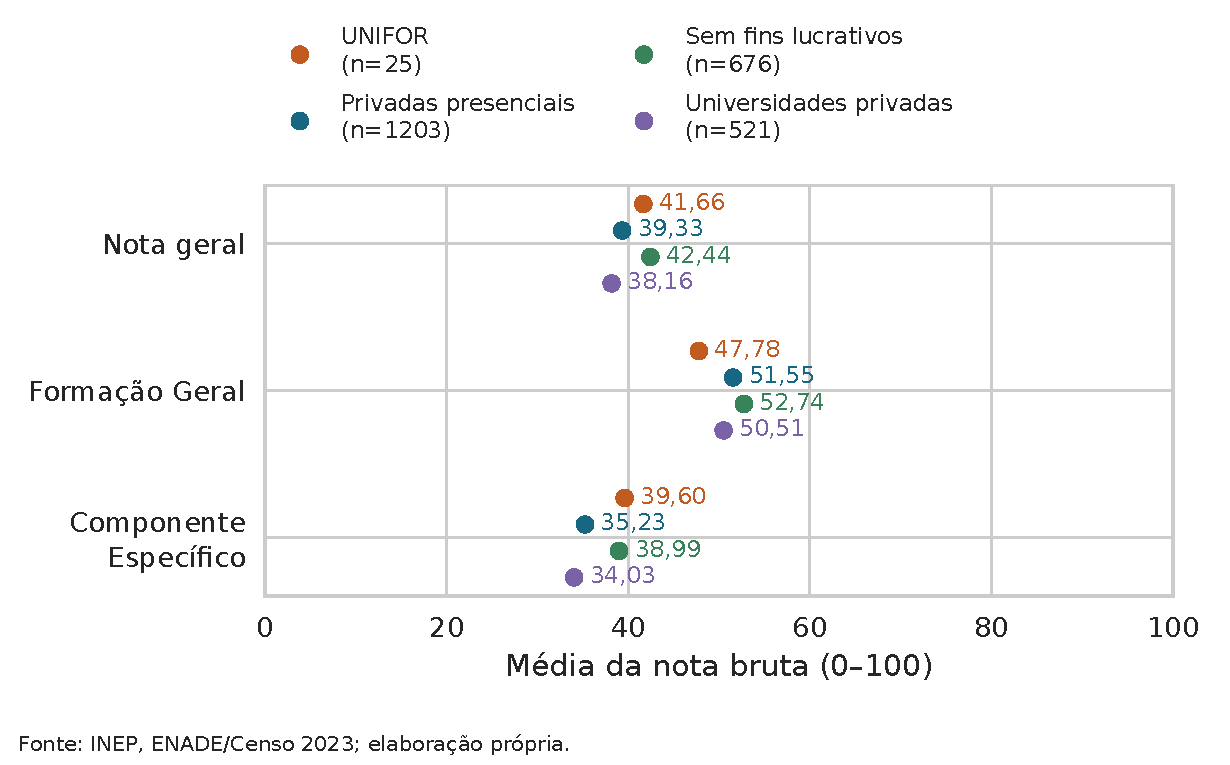
\includegraphics[width=\textwidth]{../resultados/graficos/comparacao_componentes_2023.pdf}
\caption{Médias por participante; os grupos institucionais incluem a UNIFOR e se sobrepõem.}
\label{fig:medias}
\end{figure}
A Figura~\ref{fig:medias} mostra que a UNIFOR tem média geral e CE maiores que
o universo privado, mas FG menor. Frente às privadas sem fins lucrativos, sua
média geral é menor (\MediaUniforGeral{} contra \MediaSemFinsGeral{}) e o CE
é próximo (39,600 contra \MediaSemFinsCE{}). O resultado depende do referencial
e não sustenta superioridade geral. Excluindo a UNIFOR do universo, as diferenças
descritivas são \DiferencaGeral{} pontos na nota geral, \DiferencaFG{} na FG
e \DiferencaCE{} no CE.

\subsection{FG discursiva: não resposta e notas condicionais}
\begin{figure}[H]
\centering
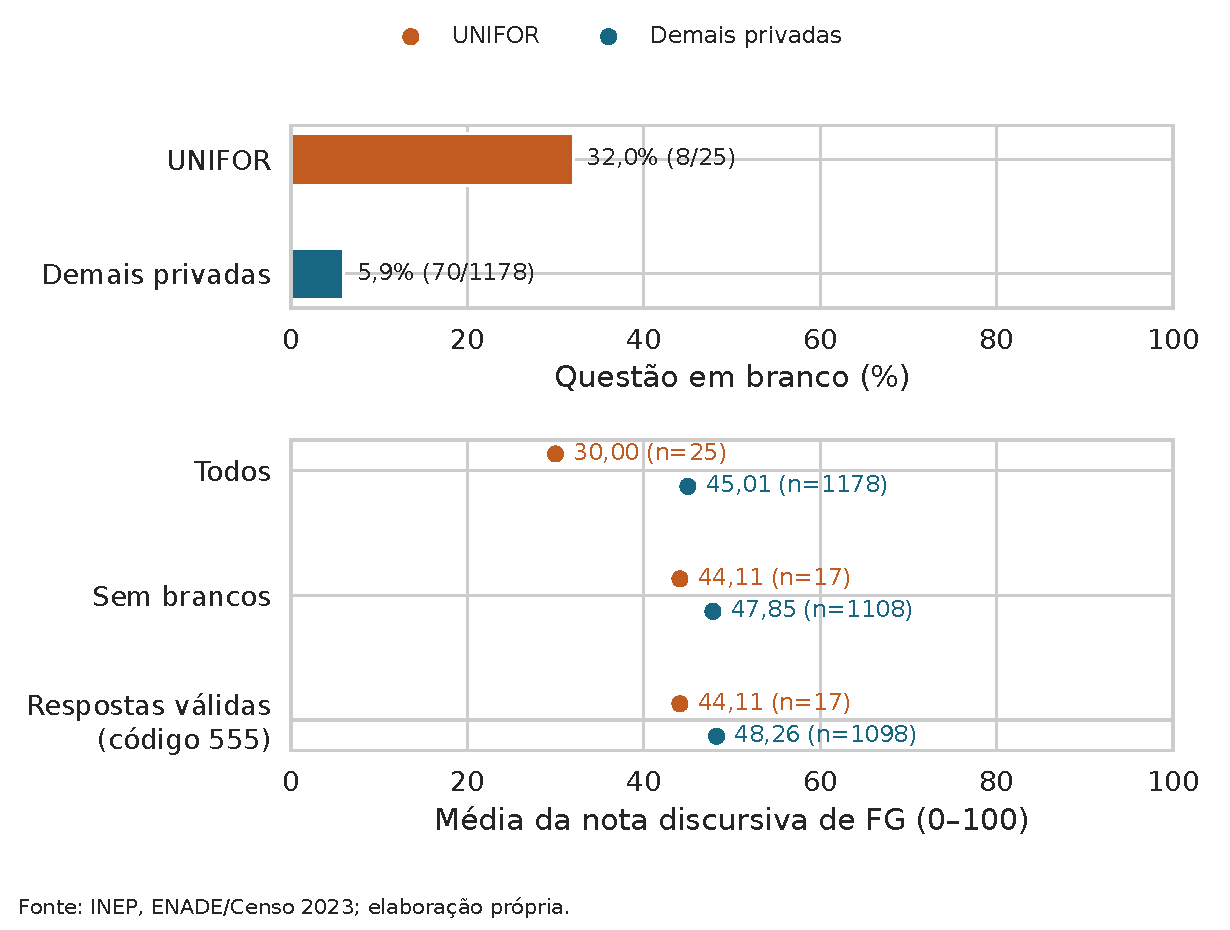
\includegraphics[width=\textwidth]{../resultados/graficos/fg_discursiva_resposta_2023.pdf}
\caption{Única questão discursiva de FG. Branco: código 333; respostas válidas: 555.
``Sem brancos'' também conserva os códigos 335/336, ausentes do último grupo.}
\label{fig:discursiva}
\end{figure}
A Figura~\ref{fig:discursiva} distingue não resposta de desempenho: há
\FGBrancosUnifor/\FGTotalUnifor{} questões em branco na UNIFOR
(\FGPercentualBrancosUnifor\%) e \FGBrancosDemais/\FGTotalDemais{} nas
demais privadas (\FGPercentualBrancosDemais\%). A média com todos é
\MediaDiscursivaFGUnifor{} contra \MediaDiscursivaFGDemais{}; entre respostas
válidas, \FGMediaRespostasValidasUnifor{} ($n=\FGRespostasValidasUnifor$)
contra \FGMediaRespostasValidasDemais{} ($n=\FGRespostasValidasDemais$).

A diferença é, portanto, muito menor no grupo com resposta válida. A maior
frequência de brancos é um componente central do contraste agregado, sem
demonstrar dificuldade de escrita, falta de conhecimento ou motivo para não
responder. Excluir apenas brancos produz \FGMediaSemBrancosUnifor{}
($n=\FGSemBrancosUnifor$) contra \FGMediaSemBrancosDemais{}
($n=\FGSemBrancosDemais$): nas demais privadas, há ainda \FGNulosDemais{}
respostas nulas (335) e \FGForaTemaDemais{} fora da temática (336).
Essas categorias não são classificadas como branco, e suas notas publicadas
são preservadas.

A FG objetiva da UNIFOR tem média \MediaObjetivaFGUnifor{}, ante
\MediaObjetivaFGDemais{}. A nota FG combina 65\% objetiva e 35\% discursiva;
CE combina 90\% e 10\%, e a nota geral pondera FG em 25\% e CE em 75\%
\cite{notaindividual}. Esses pesos reproduzem os dados arredondados e prevalecem
sobre as descrições incompatíveis 60/40 e 85/15 do XLSX local.

\subsection{Dispersão e associação FG--CE}
\begin{figure}[H]
\centering
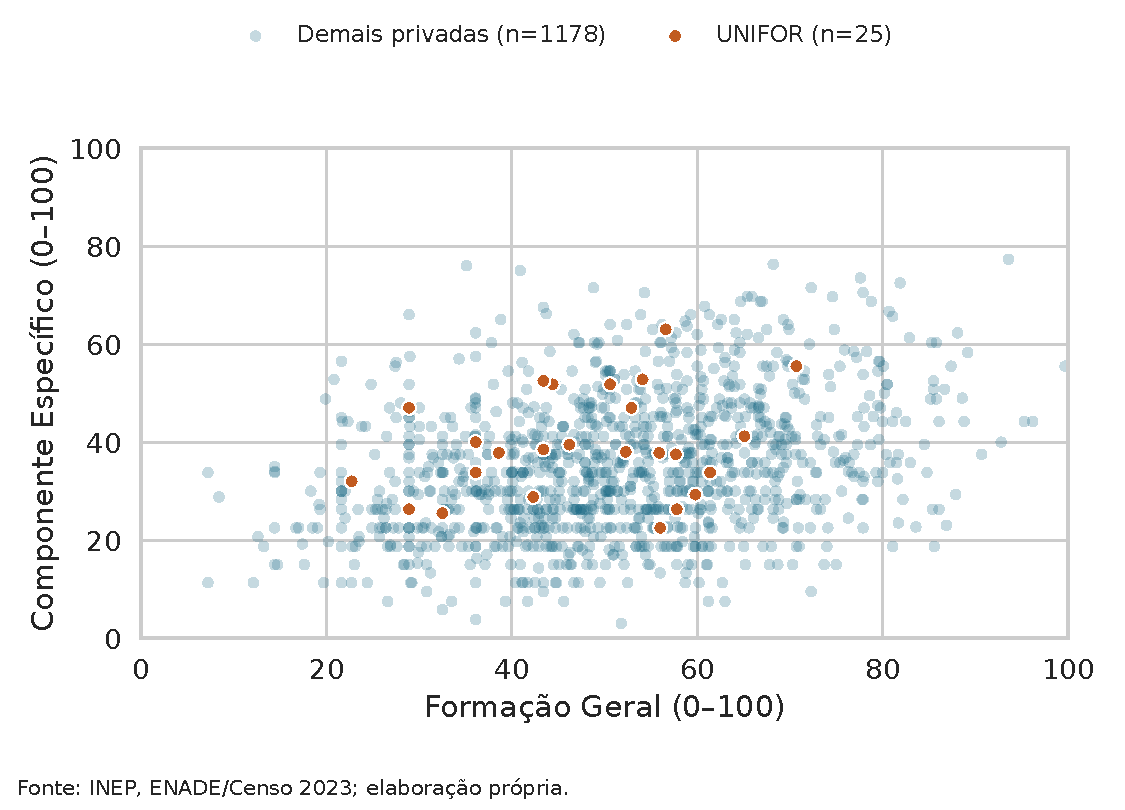
\includegraphics[width=.94\textwidth]{../resultados/graficos/relacao_fg_ce_2023.pdf}
\caption{FG e CE do mesmo registro do arq3; pontos podem se sobrepor.}
\label{fig:relacao}
\end{figure}
A Figura~\ref{fig:relacao} indica associação positiva com dispersão ampla.
Pearson é \CorrelacaoUnifor{} na UNIFOR ($n=25$), \CorrelacaoDemais{} nas
demais privadas ($n=\NotasSemUnifor$) e \CorrelacaoPrivadas{} no universo
($n=\TotalNotas$). Os DP de FG/CE são 12,37/10,72 na UNIFOR e 16,01/13,54
nas demais privadas. A amostra pequena limita a estabilidade dos resumos;
não se testou diferença entre coeficientes nem se estabeleceu causalidade.

\subsection{Questões objetivas: achados exploratórios}
\begin{figure}[H]
\centering
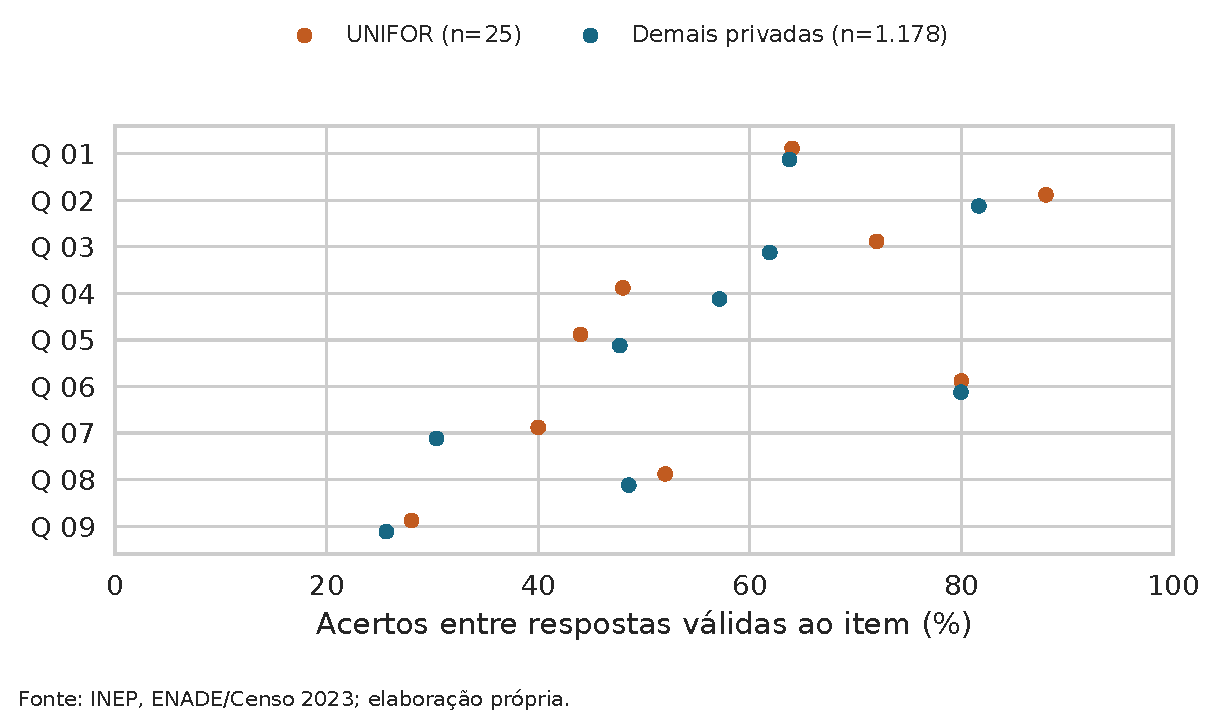
\includegraphics[width=\textwidth]{../resultados/graficos/itens_fg_2023.pdf}
\caption{Acertos nas nove questões objetivas válidas de FG; denominadores de 25 e 1.178.}
\label{fig:fg}
\end{figure}
Na Figura~\ref{fig:fg}, Q3 (72,0\% contra 61,9\%) e Q4 (48,0\% contra
57,1\%) foram destacadas por apresentarem a maior e a menor diferença
UNIFOR--demais privadas entre os itens FG. São extremos selecionados após
examinar todos os itens, portanto achados exploratórios, sem comprovação de
fragilidades específicas ou testes múltiplos. Uma resposta da UNIFOR altera
o percentual em quatro pontos percentuais.

\begin{figure}[H]
\centering
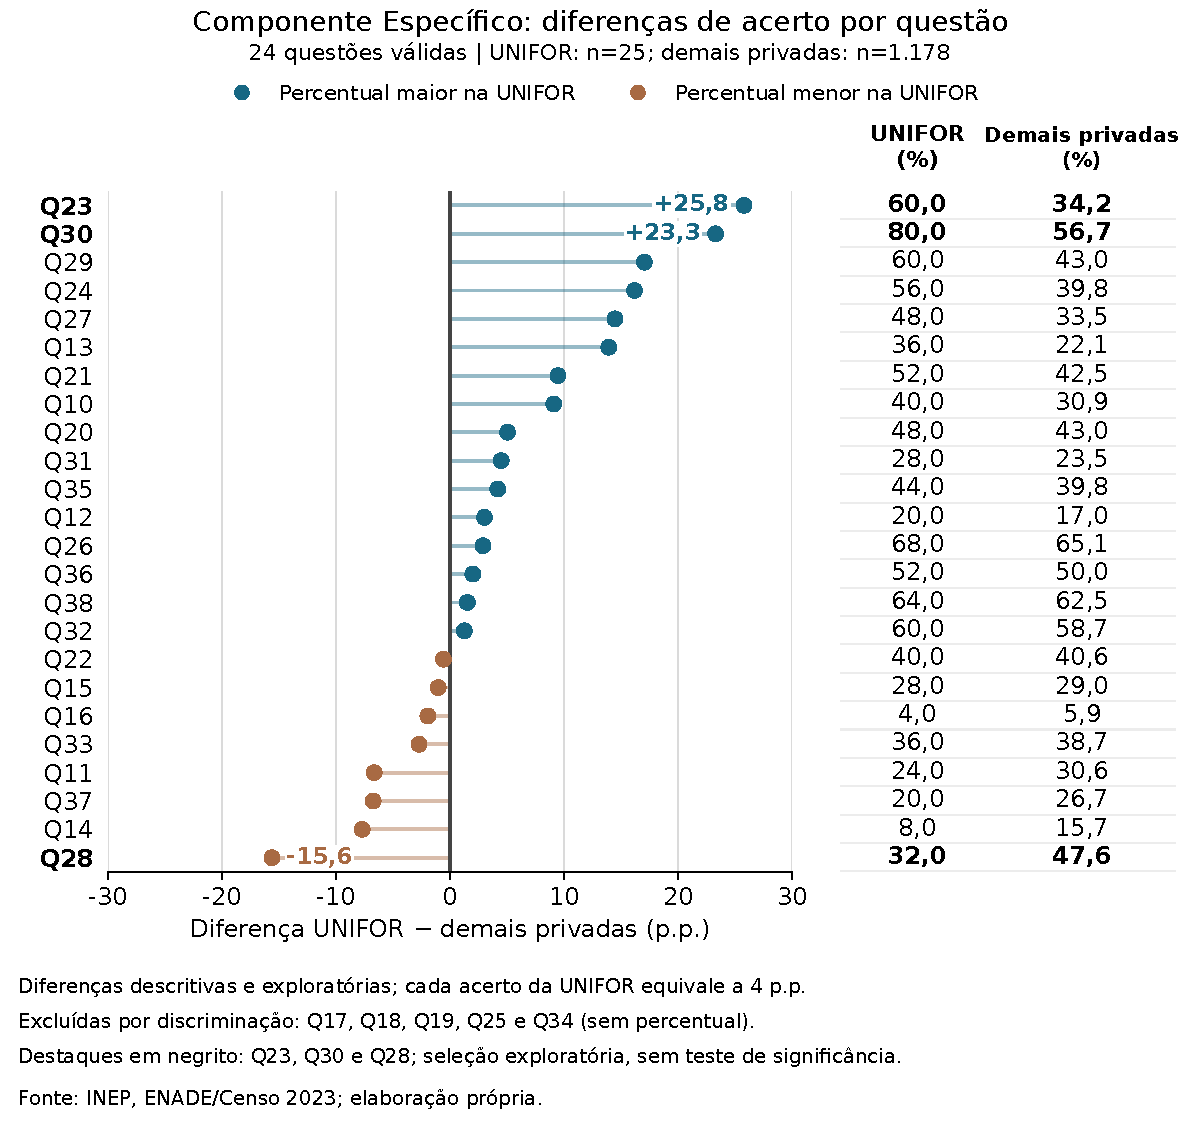
\includegraphics[width=\textwidth]{../resultados/graficos/itens_ce_2023.pdf}
\caption{Diferenças de acerto (UNIFOR menos demais privadas), em pontos percentuais,
nas 24 questões válidas de CE, ordenadas da maior para a menor.}
\label{fig:ce}
\end{figure}
A Figura~\ref{fig:ce} destaca Q23 ($+25,8$ pontos percentuais) e Q30 ($+23,3$)
como os maiores contrastes positivos, e Q28 ($-15,6$) como o maior negativo.
Os percentuais absolutos permanecem nas colunas laterais. Os destaques foram
selecionados após examinar os 24 itens válidos: são diferenças descritivas e
exploratórias, sem comprovação de significância ou fragilidades específicas.
Cada acerto representa quatro pontos percentuais entre os 25 estudantes da UNIFOR.
As cinco questões excluídas não receberam percentual zero. Escolhas, gabaritos
e acertos foram conferidos no mesmo registro, com sequência compatível com o
gabarito oficial da área \cite{gabarito}. Não se presumem questões equivalentes
entre áreas ou edições.

\subsection{Contexto socioeconômico}
\begin{figure}[H]
\centering
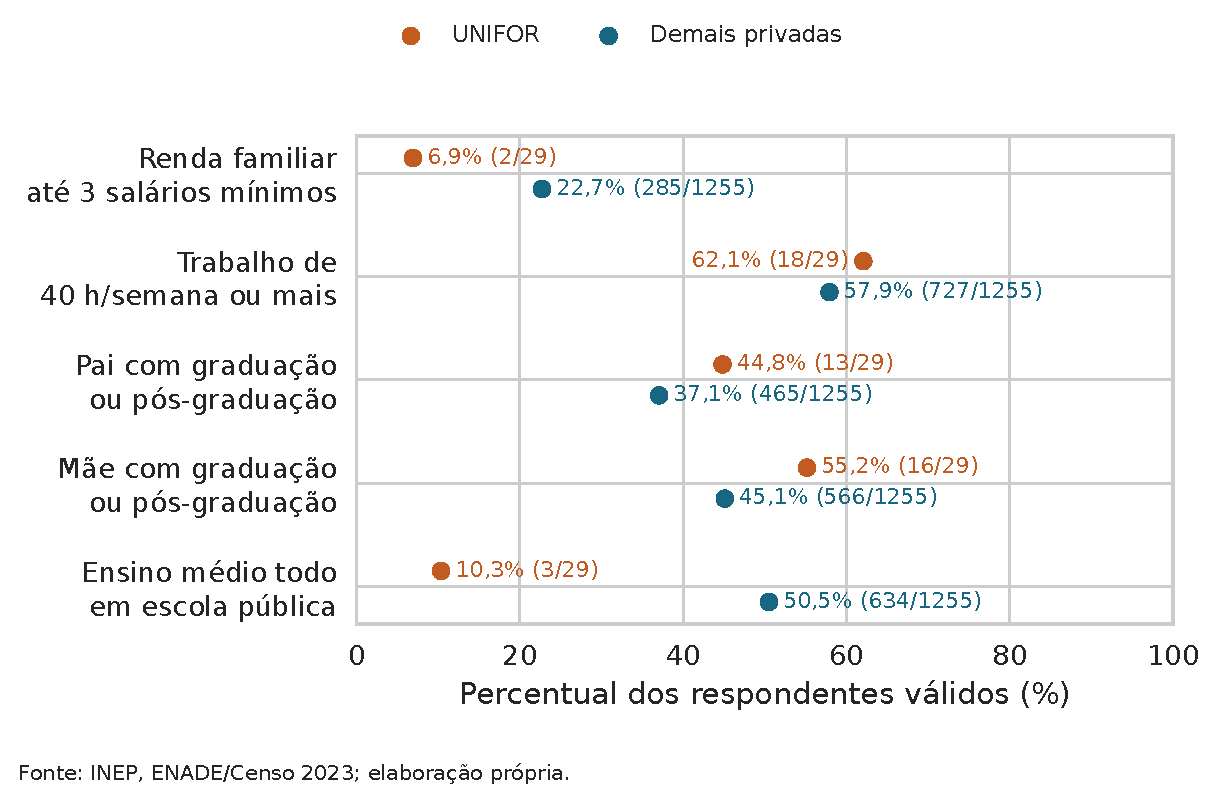
\includegraphics[width=\textwidth]{../resultados/graficos/perfil_socioeconomico_2023.pdf}
\caption{Perfis marginais por pergunta; denominadores independentes das notas. Trabalho exclui estágio e bolsas.}
\label{fig:perfil}
\end{figure}
A Figura~\ref{fig:perfil} mostra menor proporção de ensino médio integralmente
público e renda familiar até três salários mínimos na UNIFOR. Cada pergunta
tem 29 respostas publicadas e uma ausência na UNIFOR; nas demais privadas,
1.255 respostas e 133 ausências. Denominadores iguais não provam identidade
dos respondentes, nem permitem relacionar as 29 respostas às 25 notas.
As categorias seguem o questionário de 2023 \cite{questionario}.

Nos \EcoCursos{} cursos com pelo menos dez notas e dez respostas por variável,
a proporção de baixa renda e a de ensino médio todo público apresentam
associação negativa com a média geral: Pearson $r=\EcoRenda{}$ e
$r=\EcoEscola{}$, respectivamente, com peso igual por curso. A unidade é o
\textbf{curso}, não o estudante. Não existe aqui associação individual entre
renda e nota, demonstração causal ou atribuição exclusiva das diferenças ao
perfil socioeconômico. As demais correlações permanecem no notebook.

\section{Discussão, limitações e conclusão}
A UNIFOR combina CE maior que o conjunto privado com média geral menor que a
referência sem fins lucrativos. Na FG discursiva, o contraste agregado é
acentuado pela frequência maior de questões em branco; entre respostas válidas,
a diferença é menor. Não se conhecem os motivos dos brancos, e os resultados
não isolam competências de escrita ou conhecimento.

As médias descrevem notas publicadas. Sigilo, não resposta, participação e
composição dos cursos limitam a representatividade \cite[pp.~7--8]{manual}.
O curso ENADE 1125254, IES 137, permanece sem vínculo com o cadastro de cursos
do Censo, sem troca de código por semelhança. Sua categoria comunitária/confessional
é compatível com o indicador confessional, embora o indicador comunitária seja zero.
Não houve ajuste individual de notas por características de arquivos separados.

Conclui-se que distinguir participação na questão e notas condicionais evita
atribuir a menor média discursiva diretamente a uma deficiência acadêmica.
As comparações institucionais, os extremos por item e as associações por curso
são descritivos e exploratórios, sem evidência de superioridade geral ou causalidade.
A comparação com Ciência da Computação de 2021 continua pendente por ausência
de microdados locais; notas brutas de provas diferentes não mediriam diretamente
superioridade entre cursos.

\begin{thebibliography}{9}
\bibitem{enade} INEP. \textit{Microdados do ENADE 2023}.
ZIP oficial local e dicionário XLSX, versão de abril de 2025.
\href{https://www.gov.br/inep/pt-br/acesso-a-informacao/dados-abertos/microdados/enade}{Portal ENADE}.
\bibitem{censo} INEP. \textit{Microdados do Censo da Educação Superior 2023}.
Cadastros e dicionário do ZIP oficial local.
\href{https://www.gov.br/inep/pt-br/acesso-a-informacao/dados-abertos/microdados/censo-da-educacao-superior}{Portal do Censo Superior}.
\bibitem{manual} INEP. \textit{Manual do usuário -- Microdados do Enade 2023}.
Atualização de 11 abr. 2025, pp.~6--11. ZIP oficial local.
\bibitem{questionario} INEP. \textit{Questionário do Estudante Enade 2023}.
Questões 4, 5, 8, 10 e 17. ZIP oficial local.
\bibitem{notaindividual} INEP. \textit{Nota Técnica nº 12/2024/CEI/CGGI/DAES-INEP}.
Cálculo da nota individual, seção 4.
\href{https://download.inep.gov.br/educacao_superior/enade/notas_tecnicas/2024/nota_tecnica_12_calculo_nota_final_enade_2023.pdf}{Documento oficial}.
\bibitem{gabarito} INEP. \textit{Enade 2023: Engenharia da Computação -- gabarito definitivo}.
\href{https://download.inep.gov.br/enade/provas_e_gabaritos/2023_GB_engenharia_da_computacao.pdf}{Gabarito oficial}.
Exclusões estatísticas posteriores seguem o arq3.
\bibitem{conceito} INEP. \textit{Nota Técnica nº 6/2024: cálculo do Conceito Enade 2023}.
\href{https://download.inep.gov.br/educacao_superior/enade/notas_tecnicas/2024/nota_tecnica_6_metodologia_calculo_conceito_enade_2023.pdf}{Documento oficial}.
Documentos consultados em 18 out. 2026.
\end{thebibliography}
\end{document}
